\documentclass[a4paper, 11pt,addpoints]{exam}


% Margins
\topmargin=-0.45in
\evensidemargin=0in
\oddsidemargin=0in
\textwidth=6.5in
\textheight=9.0in
\headsep=0.25in 

%package usage
\usepackage[table,xcdraw,usenames,dvipsnames]{xcolor}
\usepackage[colorlinks=true, citecolor=blue, linkcolor=MidnightBlue,urlcolor=MidnightBlue]{hyperref}
\usepackage[english]{babel}
\usepackage[latin1]{inputenc}
\usepackage{indentfirst}
\usepackage{enumitem}
\usepackage{colortbl}
\usepackage{longtable}
\usepackage{threeparttablex}
\usepackage{etoolbox}
\usepackage{rotating}
\usepackage{array}
\usepackage{multirow}
\usepackage{pdflscape}
\usepackage{makecell}
\usepackage{tablefootnote}
\usepackage{makecell}
\usepackage{tabularx}
\usepackage{csquotes}
\usepackage{amssymb}
\usepackage{pifont}
\usepackage{amsmath}
\usepackage{comment}
\usepackage{flafter} 
\usepackage{dcolumn} 
\usepackage{natbib}
\usepackage{rotating}	
\usepackage{amsthm}
\usepackage{graphicx}
\usepackage{amssymb}
\usepackage{adjustbox}
\usepackage{tcolorbox}
\usepackage{lipsum}
\usepackage{tikz}
\usepackage{tabularx}
\tcbuselibrary{skins,breakable}
\usetikzlibrary{shadings,shadows}
\usepackage{threeparttable}
\usepackage{subfig}
\usepackage{setspace}
\usepackage{booktabs}
\usepackage{placeins}
\usepackage{enumitem}
\usepackage[encoding,filenameencoding=utf8,extendedchars,space]{grffile}
\newcommand{\addfig}[2]{\begin{center}
			\includegraphics[width=#1\textwidth]{#2}
	\end{center}
}

%\usepackage[capposition=top]{floatrow}
%\usepackage[colorinlistoftodos]{todonotes}
\newcommand{\expect}[2]{\mathbb{E}_{#2}\left(#1\right)}
\newcommand{\explaino}[2]{\overbrace{#1}^{\text{\textbf{#2}}}}

\newtheorem{theorem}{Theorem}[section]
\newtheorem{corollary}{Corollary}[theorem]
\newtheorem{proposition}[theorem]{Proposition}

\newcommand{\alert}[1]{{\textbf{\color{red}#1}}}
%general commands
\newcommand{\beqns}{\begin{eqnarray*}}
\newcommand{\eeqns}{\end{eqnarray*}}
\newcommand{\beqn}{\begin{eqnarray}}
\newcommand{\eeqn}{\end{eqnarray}}
\newcommand{\benu}{\begin{enumerate}}
\newcommand{\eenu}{\end{enumerate}}
\newcommand{\bitem}{\begin{itemize}}
\newcommand{\eitem}{\end{itemize}}
\newcommand{\smallGap}{\vspace{.25cm}}
\newcommand{\oemph}[1]{\textbf{\orange{#1}}}

\newenvironment{block}[1]{%
	\tcolorbox[beamer,%
	noparskip,breakable,
	colback=LightGreen,colframe=DarkGreen,%
	colbacklower=LimeGreen!75!LightGreen,%
	title=#1]}%
{\endtcolorbox}


\newcommand{\sym}[1]{\rlap{#1}}% Thanks David Carlisle

\usepackage{siunitx}
\sisetup{
	detect-mode,
	group-digits		= false,
	input-symbols		= ( ) [ ] - +,
	table-align-text-post	= false,
	input-signs             = ,
}

%mathematical commands

\newcommand{\cov}{\text{cov}}
\newcommand{\var}[1]{\text{var}\left(#1\right)}
\newcommand{\red}[1]{{\color{red}#1}}
\newcommand{\blue}[1]{\color{blue}{#1}}
\newcommand{\green}[1]{{\color{Green}#1}}

\newcommand{\vs}{\vspace{1mm}}
\usepackage{framed}
\definecolor{shadecolor}{gray}{0.875}
\specialcomment{answer}{\begin{shaded}}{\end{shaded}}
\newcommand{\PreserveBackslash}[1]{\let\temp=\\#1\let\\=\temp}
\newcolumntype{C}[1]{>{\PreserveBackslash\centering}p{#1}}
\newcolumntype{R}[1]{>{\PreserveBackslash\raggedleft}p{#1}}
\newcolumntype{L}[1]{>{\PreserveBackslash\raggedright}p{#1}}
\newcommand{\thesispath}{..}
\usepackage{titlesec}
\usepackage{breakurl}
\urlstyle{same}
\usepackage{float}
\usepackage{natbib}
\usepackage{listings}



\onehalfspacing



\newcommand{\questionpoints}[1]{
	\par\noindent\textbf{[#1 mark(s)]}
}

\title{\large{\textbf{ECNM10112: Applied Labour Economics}}}
\author{\textbf{Empirical Group Project}}
\date{\textbf{Due date:} \red{\textbf{Thursday,  6  November at 3 pm}}}
\begin{document}
\maketitle

\noindent\textbf{General guidelines:} This group project is based on the paper \href{https://academic.oup.com/qje/article/130/2/571/2330321}{Gender Identity and Relative Income within Households} by Marianne Bertrand, Emir Kamenica and Jessica Pan\nocite{Bertrand2015}. You will use publicly available data from IPUMS United States to produce some parts of the paper. Please follow the general guidelines below:

\bitem 
\item You will work in \textbf{pairs}. \textbf{Each pair will submit a unique handout and set of code.}
\item Please include both your group and exam numbers on the cover of your handout. \textbf{Do not write your names in your handout}.
\item This project consists of \textbf{7 questions}. \textbf{You need to answer all questions}. You should produce a document containing the answers to all these questions, including tables and figures.
\item \textbf{Keep all answers to questions 1 to 6 to at most 130 words}. The word limit excludes text in figures, equations, and tables. Violations of this limit will be penalised.
\item Each group should submit a unique \textbf{pdf} file containing all their answers and another file containing all their code to LEARN. Please do not paste code into the pdf file you submit. \textbf{Only one person per group should submit}.
\item There will be \textbf{one submission} box on Learn where you will submit two files: 
\bitem 
\item The \textbf{pdf} file with all your answers (including tables and figures).
\item A \textbf{zip} file containing all your code. The zip file will contain all the scripts you used to generate your results. \textbf{Do not} include any of the data files in the zip file.
\eitem 
\item Please name your pdf and zip file as follows: {\tt handout\_G[group number].pdf} and \\ {\tt code\_G[group\_number].zip}. For example, files for group 1 should be called {\tt handout\_G01.pdf} and {\tt code\_G01.zip}.
\item Tables and figures should be appropriately labelled and they should look professional and self-explanatory. Marks will be subtracted for tables with cryptic information or screenshots from the Stata command window (or the relevant equivalent for the software you used).
\item All your code should be reasonably commented so that an outsider would be able to make out what the code does. Your code should reproduce all the results that you include in the pdf.
\item You are free to use any software or code language you feel most comfortable with, but solutions will only be provided with Stata code.
\item Please note that your estimates will not exactly reproduce the numbers shown in the paper. Although they should look ``qualitatively'' similar, they will not match exactly. Do not waste time and energy trying to make your estimates match exactly those in the paper.
\item \textbf{Free riding:} This is a group project; you are responsible for dividing and coordinating work among yourselves. Refer to the \href{https://www.learn.ed.ac.uk/ultra/courses/_121272_1/outline/edit/document/_10205264_1?courseId=_121272_1&view=content}{course outline} for guidance if a group member is free riding.
\item \textbf{Plagiarism and AI:} 
\bitem 
\item All answers and code you submit must be your own work. Presenting work you did not do as your own without appropriate acknowledgment is plagiarism. Any suspicion of plagiarism will be investigated and sanctioned in accordance with school policy. 
\item We allow the use of generative AI tools (such as ChatGPT, GitHub/Microsoft Copilot, or similar) as a means to brainstorm or troubleshoot your code. Any use of these tools should be acknowledged in your submission. Note, however, that presenting AI-generated answers as your own, be that code or text, is plagiarism and will be sanctioned accordingly. See the \href{https://information-services.ed.ac.uk/computing/communication-and-collaboration/elm/generative-ai-guidance-for-students/using-generative}{university guidance on AI} for additional information.
\eitem 
\eitem 
\newpage 
\section*{Part I: cleaning the data}
\noindent In this first part, you will work on cleaning data from the US Censuses and the American Community Survey (ACS).
\bitem
	\item Please download the zip file corresponding to your group from \href{https://www.dropbox.com/scl/fo/g2xtn0yymiebz0wivfe7k/AGwxkhhcV-4sBT43u8ZHYL4?rlkey=a8g768pa9m9v067bg9pudg10h&dl=0}{this folder} and decompress it.
	\item You will find two files:
	\bitem 
		\item ex\_[group number]\_census\_acs.dta (Stata format)
		\item census\_codebook.pdf
	\eitem 
	The data file contains random samples from the 1990 and 2000 US Decennial Census and the 2008-2011 American Community Survey (ACS) \citep{IPUMS}. If you are using other software, you can easily export the file to csv using Stata. The pdf file contains variable descriptions and code dictionaries.
	
	The data was extracted from the 5\% 1990 and 2000 census samples, and the 3-year ACS for 2011 (see \burl{https://usa.ipums.org/usa-action/samples}). \textbf{For simplicity, I will refer to the 2008-2011 ACS as the 2011 data.}
	
	All variables keep the original names and labels from IPUMS.  Additional data documentation can be found at \burl{https://usa.ipums.org/usa-action/variables/group}. Just search for the variable you want and click on the variable name on the search results. When you click on the variable name, you will be on a site similar to the one shown in the screenshot. There is an analogous page for each variable in the dataset. The codes tab shows a description of the meaning of each variable value, universe indicates the set of people to whom each question was asked, and questionnaire text shows you the actual question that was asked to the respondent. 
	
	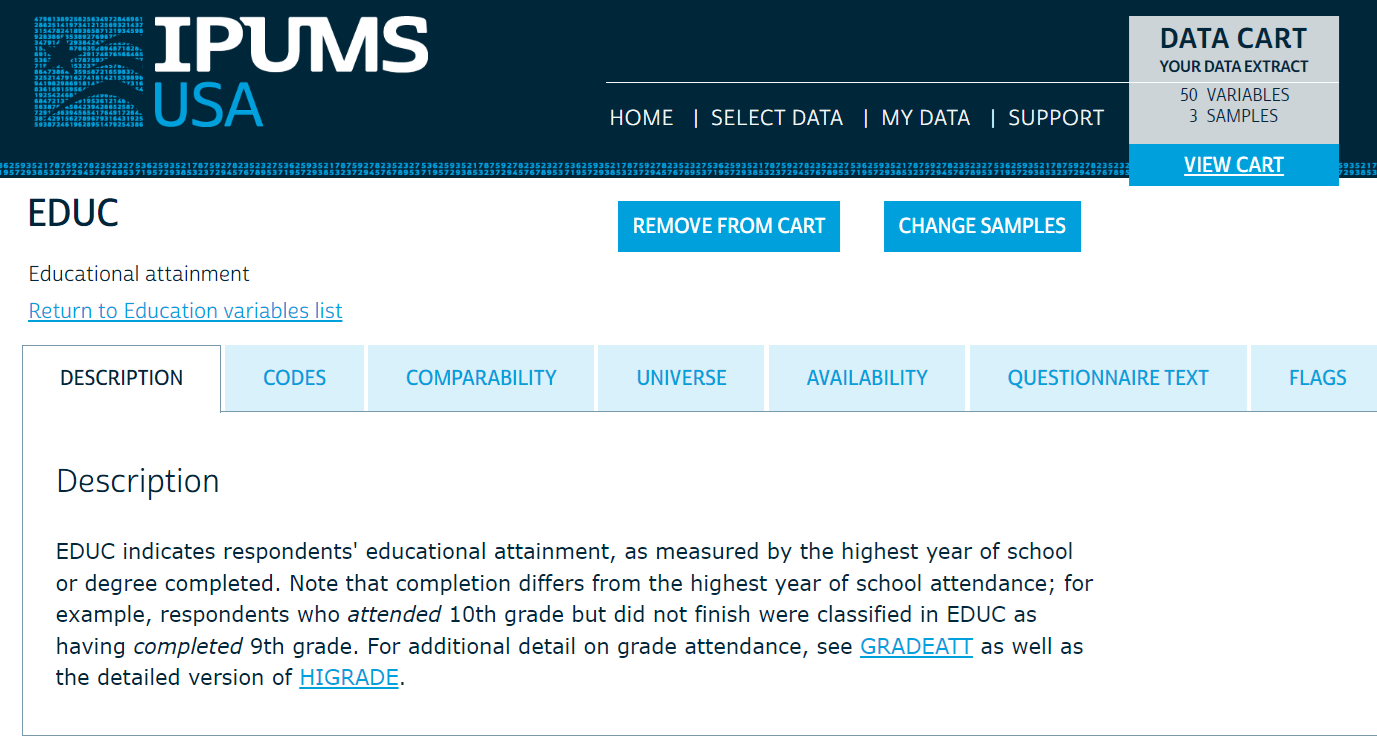
\includegraphics[width=.9\textwidth]{screenshot_educ.png}
\eitem 
\newpage
\begin{questions}
	\question[5] 	
	Please provide in \textbf{your own words} a short summary of the paper.  
	\question[15] \label{clean:first} Filter and clean the data using the following steps (in this order):
	\begin{enumerate}[label=(\alph*)]
		\item Keep only heads of household and their spouses.
		\item Drop anybody with negative values in any of the income variables.
		\item Keep only people aged between 18 and 65 years old (inclusive).
		\item Drop people with imputed income components. The imputation flags are named as follows: Q[VARIABLE NAME]. For example, the imputation flag for INCWAGE is QINCWAGE.\label{step:first}
		\item Restrict the data to complete couples, i.e. households with a household head and a spouse.
		\item For each income component: \label{step:last}
		\bitem 
		\item Drop couples where both members have top-coded values.  Top-coding is common for income information to preserve confidentiality. See \href{https://faculty.chicagobooth.edu/-/media/faculty/emir-kamenica/documents/identityonlineappendix.pdf}{here} for details.
		\item For couples where only one spouse has top-coded income, multiply his/her income by 1.5 and leave the other individual's income as is.
		\eitem 
		\item Compute total personal income by summing all income components. See \href{https://usa.ipums.org/usa-action/variables/INCTOT#comparability_section}{here} for details on which variables you need to use.
		\item Keep only heterosexual couples.
		\item Compute the individual's share in the couple's income as:
		\beqn
			{\tt income\_share}=\frac{total\text{ }personal\text{ }income}{husband's\text{ }income+wife's\text{ }income}
		\eeqn
	\end{enumerate}
	After you have applied these procedures, complete table \ref{tab:table_1_empty} using your data.
	
	\begin{center}
\begin{adjustbox}{max width=.9\textwidth}
\begin{threeparttable}[H]
\caption{Summary statistics for individual-level data}
\label{tab:table_1_empty}
\begin{tabular}{lrrrrrrrrr}
\toprule
\toprule
\textbf{}&\multicolumn{1}{c}{\textbf{1990}}&\multicolumn{1}{c}{\textbf{2000}}&\multicolumn{1}{c}{\textbf{2011}} \\
\midrule
Number of people & ... & ... & ... \\ 
Mean age  & ... & ... & ... \\ 
Share female   & ... & ... & ... \\ 
Share non-white  & ... & ... & ... \\ 
Share with some college  & ... & ... & ... \\ 
Mean total income    & ... & ... & ... \\ 
\bottomrule
\bottomrule
\end{tabular}
\end{threeparttable}
\end{adjustbox}
\end{center}

	
	\begin{solution}
		\begin{center}
\begin{adjustbox}{max width=.9\textwidth}
\begin{threeparttable}[!h]
\caption{Individual summary statistics}
\label{tab:table_1}
\begin{tabular}{lrrrrrrrrr}
\toprule
\toprule
\textbf{}&\multicolumn{1}{c}{\textbf{1990}}&\multicolumn{1}{c}{\textbf{2000}}&\multicolumn{1}{c}{\textbf{2011}} \\
\midrule
Number of people & 1,447,140 & 1,192,938 &   899,782 \\ 
Mean age &     41.32 &     42.61 &     45.87 \\ 
Share female &      0.50 &      0.50 &      0.50 \\ 
Share non-white &      0.12 &      0.16 &      0.16 \\ 
Share with some college &      0.51 &      0.53 &      0.61 \\ 
Mean total income & 23,793.53 & 38,811.48 & 50,927.86 \\ 
\bottomrule
\bottomrule
\end{tabular}
\begin{tablenotes}
\item \footnotesize \textit{Notes:} Table shows summary statistics for the full sample. 
\end{tablenotes}
\end{threeparttable}
\end{adjustbox}
\end{center}

	\end{solution}	
	
	\question[15] The authors spent a lot of time trying to deal with a spike in the couple's distribution of relative income. Explain why this spike might be worrying for their exercise. Does the spike remain present after you applied all the cleaning steps from question \ref{clean:first}? Use a histogram to illustrate it. Your histogram will look nicer if you plot only women with non-zero income.
	\begin{solution}
	The problem main problem is that there is a big spike of couples where the share of income is exactly 0.5.  This big spike does appear in Figure \ref{fig:figure_1}. The whole idea of the paper is arguing that there is ``something'' special about women earning slightly more than their husbands. To argue this you need couples just below and just above the 0.5 income share cutoff to the be similar. This becomes harder to argue when there is something else going on at 0.5, which is what the histogram seems to suggest. 
	\begin{figure}[H]
\centering
\caption{Share of couples by women's relative income}
\label{fig:figure_1}
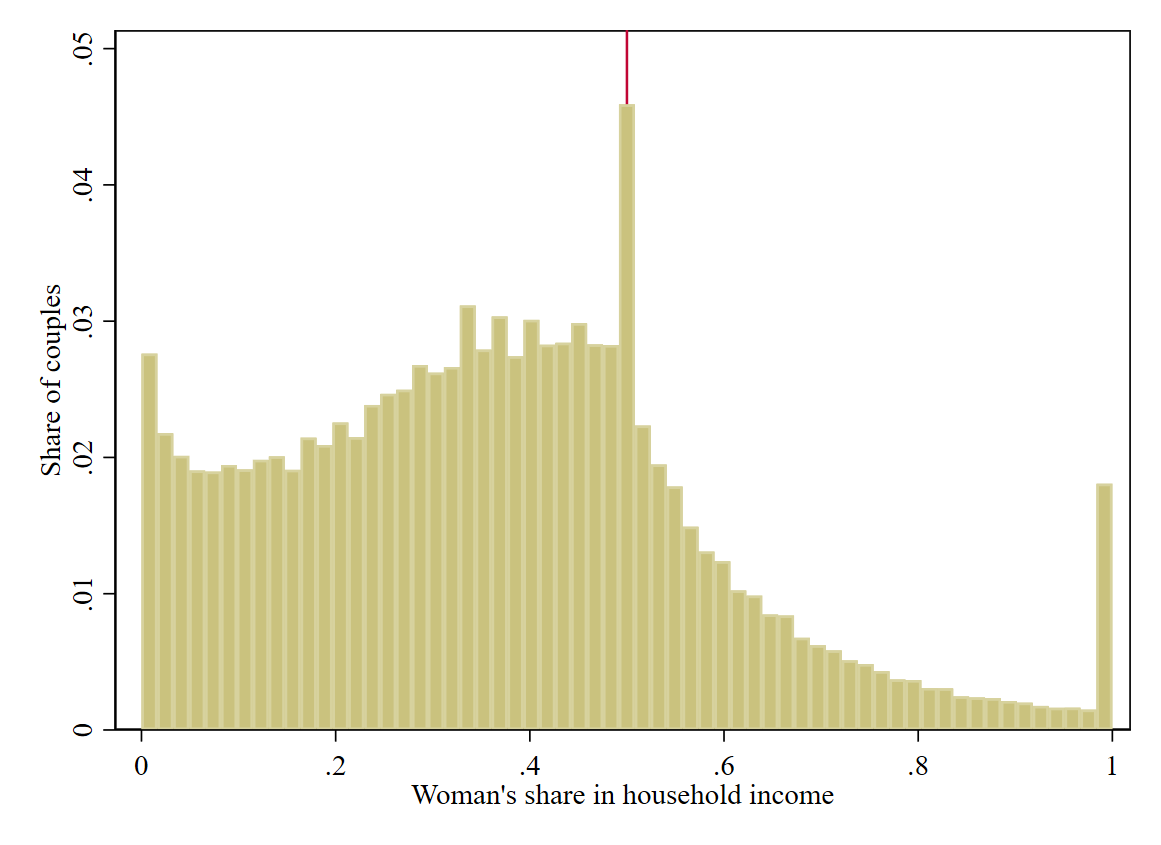
\includegraphics[width=.5\textwidth]{../../results/figures/figure_1.png}
\par \begin{minipage}[h]{\textwidth}{\scriptsize\textit{Notes:} For readibility the histogram restricts couples where women have non-zero income. Vertical line marks couples where the woman earns 50\% of the couples income.}\end{minipage}
\end{figure}

	\end{solution}
	\FloatBarrier
	\question[15] The authors show that some of the residual data issues come from the rounding of incomes by IPUMS. For confidentiality purposes, IPUMS sometimes rounds incomes to multiples of USD 100. The authors take a lot of care to ``undo'' the rounding. However, their (careful) procedure is too cumbersome for the objectives of this assignment. We will cheat and do a much simpler procedure that will achieve a similar result. We will add random noise to some women's income.
	\label{question:noise}
	\benu[label=(\alph*)]
		\item Set the random seed to 100 [\href{https://stats.oarc.ucla.edu/stata/faq/how-can-i-draw-a-random-sample-of-my-data/#:~:text=Setting%20the%20seed&text=The%20seed%20is%20the%20number,command%20followed%20by%20a%20number}{Stata}] [\href{https://r-coder.com/set-seed-r/}{R}]. Setting the seed guarantees that your results are. \textbf{Set the seed in your do file, don't do it manually. If you don't set the seed, you will get different results every time you run your code}.
		\item Generate a dummy called {\tt target\_women} equal to one for women satisfying both these conditions:
		\bitem 
			\item They have non-zero income.
			\item Their relative share of the couple's income is between 0.49 and 0.51 (inclusive).
 		\eitem   
 		\item \label{item:addnoise} We will add  income noise to 40\% of the women satisfying the conditions above. We will choose these women randomly. To do so:
		\bitem 
		\item Generate a uniform random number between 0 and 1 for women with {\tt target\_women} equal to one. 
		\item We will add noise to women whose random number is lower than or equal to 0.4. Flag these women with the dummy variable {\tt flag\_noise}.
		\item Generate the variable {\tt income\_noise} as follows:
		\begin{quote} 
			{\tt
			generate income\_noise=exp(rnormal(0,1.14)) if flag\_noise==1 \\
			replace  income\_noise=1 if missing(flag\_noise)|flag\_noise==0
		}
		\end{quote}
		\item Add the noise to the income as follows:
		\begin{quote} 
			{\tt
				generate noise\_inctot=inctot * income\_noise
			}
		\end{quote}
		\eitem 
	\eenu 
	Recompute the income share using {\tt noise\_inctot} and plot it in a histogram. Your histogram will look nicer if you plot only women with non-zero income. Why do you think it is important that we randomly selected the women we added income noise in \ref{item:addnoise}?
	\begin{solution}
		Figure \ref{fig:figure_2} shows that adding noise to the wife's income made the spike at 0.5 disappear, which is what the authors wanted to solve. It is important to select the women randomly to ensure we did not introduce selection bias into our exercise.
	
		\begin{figure}[H]
\centering
\caption{Share of couples by women's relative income (after adding noise to wife's income)}
\label{fig:figure_2}
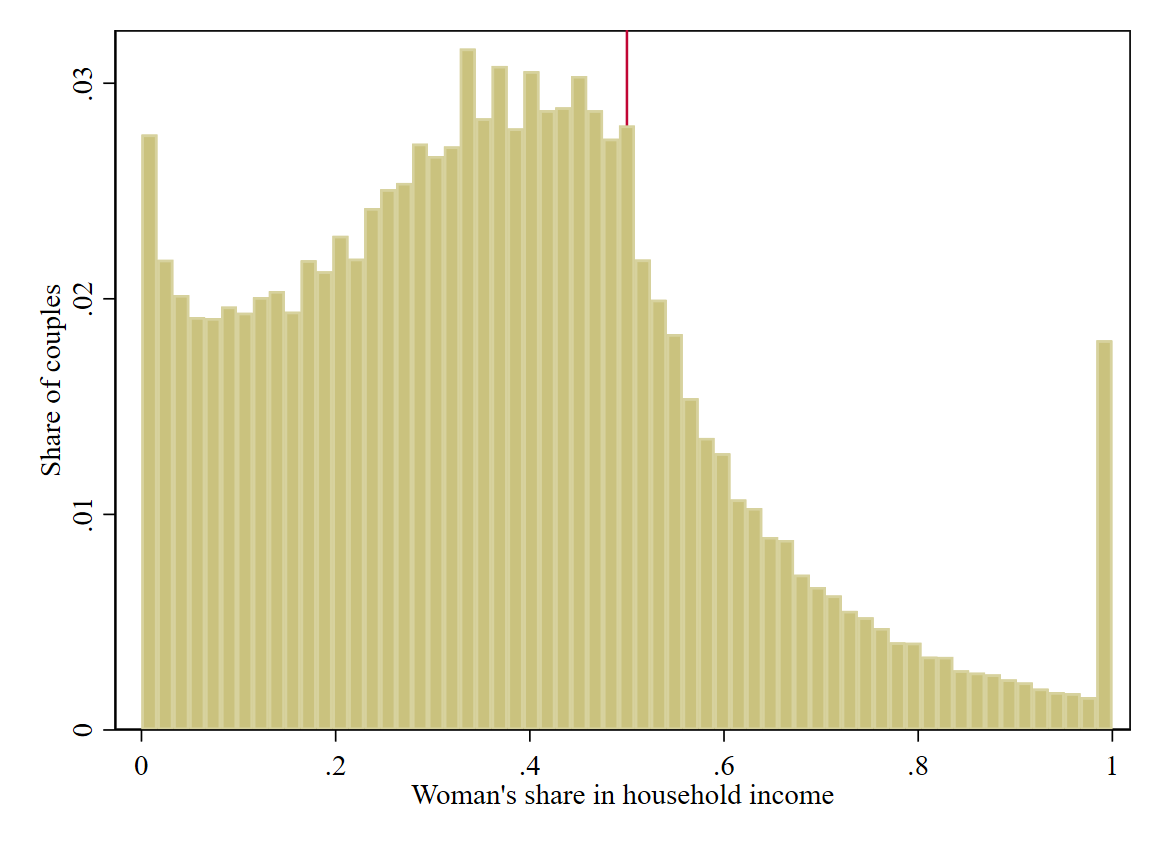
\includegraphics[width=.5\textwidth]{../../results/figures/figure_2.png}
\par \begin{minipage}[h]{\textwidth}{\scriptsize\textit{Notes:} For readibility the histogram restricts couples where women have non-zero income. Vertical line marks couples where the woman earns 50\% of the couples income.}\end{minipage}
\end{figure}

	\end{solution}
\newpage
\section*{Part II: RDD}
\noindent \textbf{In this second part, you will use the data you cleaned in part I to do a Regression Discontinuity exercise. We will cover RD on week 6. Quick notes are available \href{https://cesarlgm.github.io/documents/teaching/labour_documents/rdd_notes.pdf}{here}. \newline \newline For this second part, drop couples where the wife has zero income. All calculations should be made using the corrected income share you computed  in question (\ref{question:noise})}
\question[15] We will first make a visual version of the RDD. This is a replication of Figure III in the paper. To do so:
\bitem 
\item Group wife's share of income into bins of width 0.05 that include the top of the interval. For example: the first bin includes shares of income from 0 to 0.05 (inclusive). The second includes shares \textbf{strictly greater than} 0.05 and \textbf{lower or equal to} 0.1, and so on and so forth.
\item Collapse / aggregate your data at the bin-year level. When aggregating, compute the count of couples in each bin-year cell.
\item Compute a new variable showing, for each year, the share of couples that belong to each income share bin.
\item Reproduce Figure III for the years 1990, 2000, and 2011. Example code to produce similar graphs is available \href{https://cesarlgm.github.io/documents/teaching/labour_documents/code_example_lowess.pdf}{here}. Evidently, you will need to adjust the code to suit your purposes. \textbf{Be aware that, while similar, there will be some differences between your figure and the paper's.}
\eitem 
Explain \textbf{in your own words} what the graphs you produced show.
\begin{solution}
	Figure \ref{fig:figure_3} shows  a clear drop in the in share of couples where the woman makes just a bit more than the man. This suggests that there is an aversion to form or stay in couples where the woman is the highest earner.
	\begin{figure}[H]
\centering
\caption{Share of couples by women's relative income by year}
\label{fig:figure_3}
\subfloat[1990]{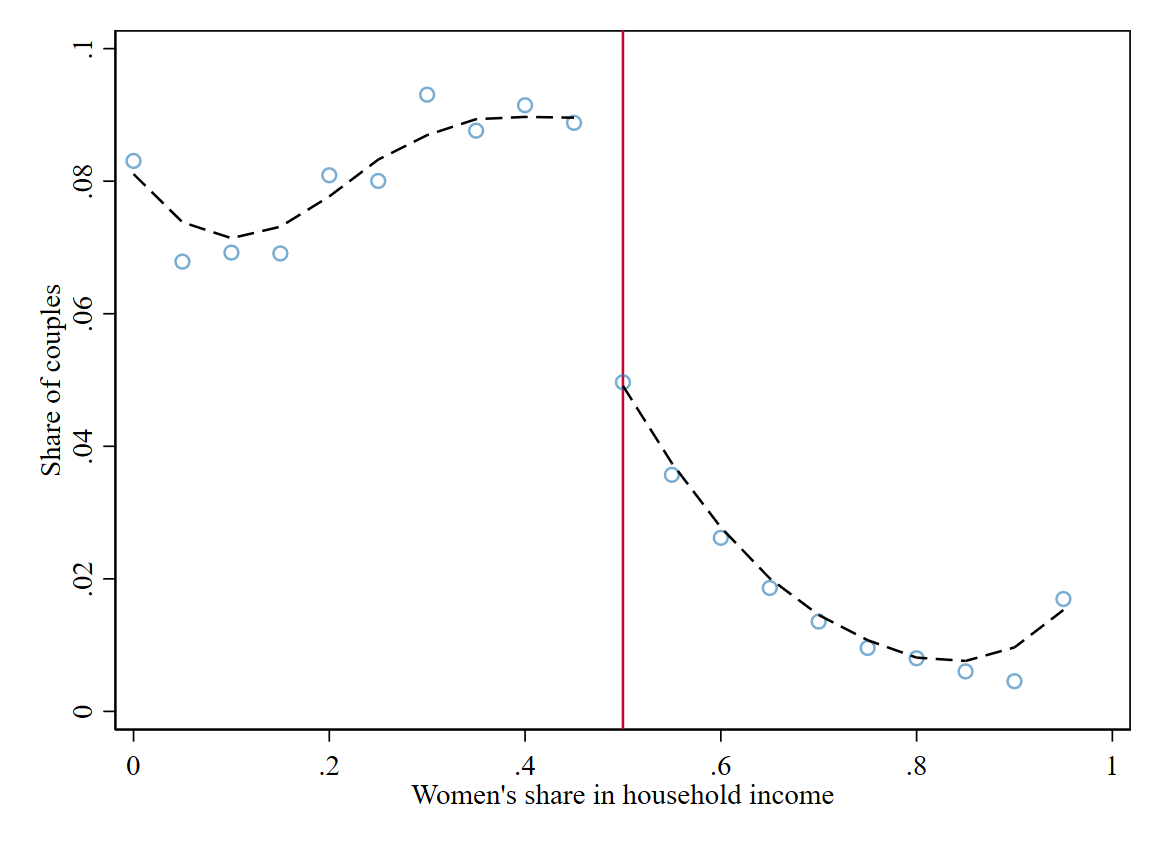
\includegraphics[width=.5\textwidth]{../../results/figures/figure_3_1990.png}} \subfloat[2000]{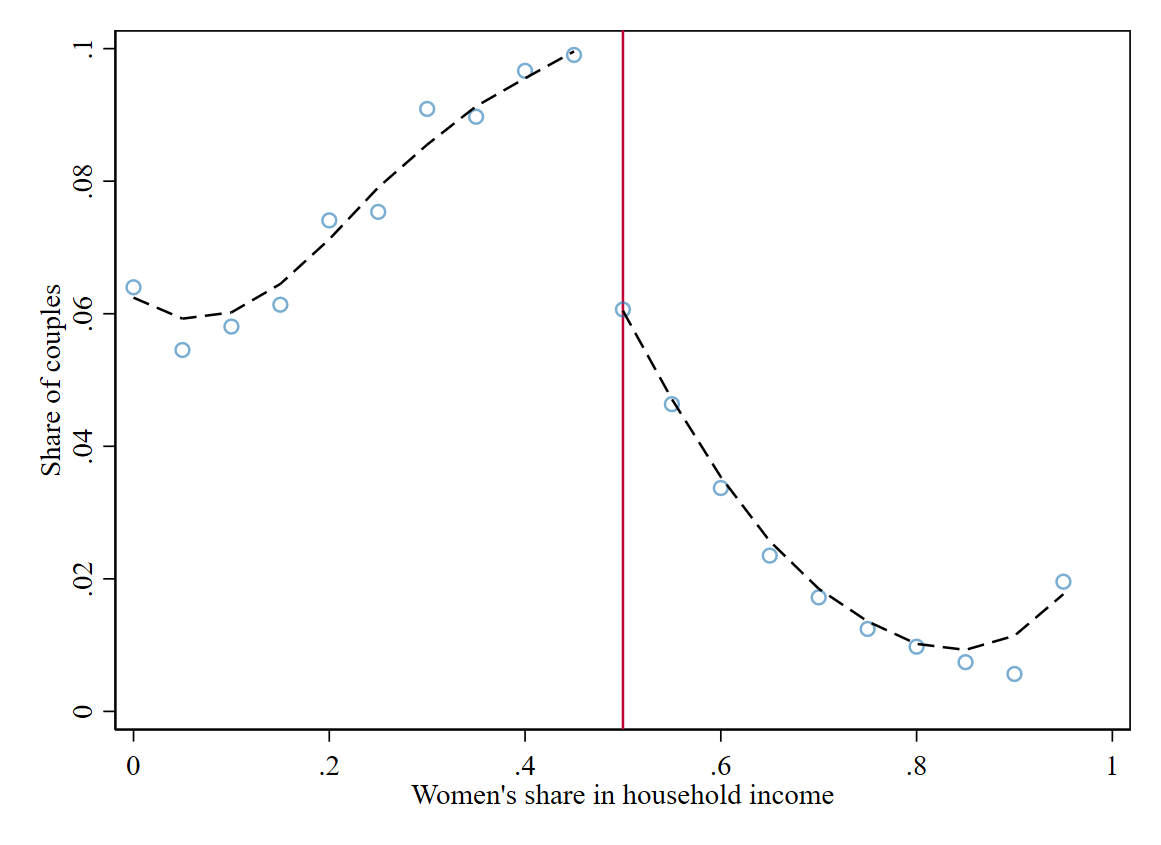
\includegraphics[width=.5\textwidth]{../../results/figures/figure_3_2000.png}} \\ \subfloat[2011]{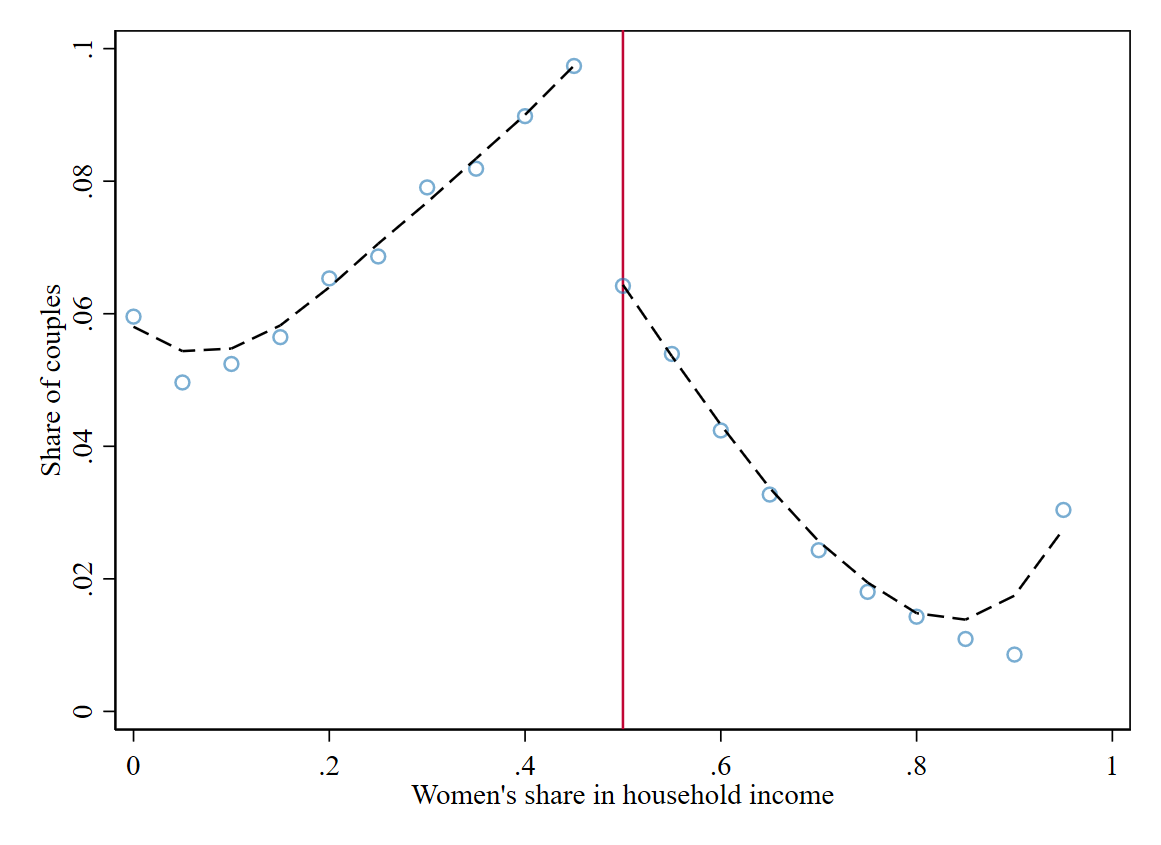
\includegraphics[width=.5\textwidth]{../../results/figures/figure_3_2011.png}} 
\par \begin{minipage}[h]{\textwidth}{\scriptsize\textit{Notes:} Each dot represents a bin of size 0.05 of the relative income share. Vertical line marks couples where the woman earns 50\% of the couples income.}\end{minipage}
\end{figure}

\end{solution}
\question[20] Now you will create the regression analogue of the figures from the previous question. To do so:
\label{eq:reg_table}
\bitem 
	\item Go back to the individual-level data. Group wife's share of income into bins of 2.5 percentage points width and collapse/aggregate it by year and bin. When aggregating it, compute the count of the number of couples.
	\item Compute a new variable showing, for each year, the share of couples that display a particular income share value. Call this variable {\tt share\_couples}.
	\item Estimate a RD regression using {\tt income\_share} as running variable and  {\tt share\_couples} as dependent variable. Include linear, quadratic, and cubic terms of the running variable. Set the discontinuity at 50\% of relative income. Compute a unique estimate for the whole period (i.e. do not compute estimates by decade) and allow for different functional form on each side of the discontinuity.
\eitem 
Interpret \textbf{using your own words} the estimate of the discontinuity term. Is it statistically significant? Explain in your own words what do you need to assume to interpret this estimate in a causal way.
\begin{solution}
	Table \ref{tab:table_2} shows estimates of the women discontinuity dummy in the regression: 
	\beqns
		share\_couples_{it}&=&\beta_0+\tau D_{it}+\beta_1*wife\_share_{it}+\beta_2*wife\_share_{it}^2+\beta_3*wife\_share_{it}^3\\
		&&+\beta_4 D_{it}(wife\_share_{it}-.5)+\beta_5 D_{it}(wife\_share_{it}-.5)^2\\
		&&+\beta_5 D_{it}(wife\_share_{it}-.5)^3)+\varepsilon_{it}
	\eeqns
	where $D_{it}$ is a dummy equal to one if the wife's share of income is greater than 0.5. The estimate indicates that the likelihood of observing a couple where the wife makes just slightly more than the husband is 1.6 p.p. lower than one in which the wife makes just slightly less than the husband. This drop is significant at the 1\%.
	
	\begin{center}
\begin{adjustbox}{max width=.9\textwidth}
\begin{threeparttable}[H]
\caption{Regression discontinuity estimates}
\label{tab:table_2}
\begin{tabular}{lrrr}
\toprule
\toprule
\textbf{}&\multicolumn{1}{c}{(1)} \\
\midrule
Woman is the highest earner&      -0.016\sym{***}\\
                    &     (0.003)         \\
\midrule Observations&     120.000         \\
\bottomrule
\bottomrule
\end{tabular}
\begin{tablenotes}
\item \footnotesize \textit{Notes:} The regression includes a cubic polynomical of the relative income share, along with interactions between the discontinuity and the polynomial. 
\end{tablenotes}
\end{threeparttable}
\end{adjustbox}
\end{center}

\end{solution}
\question[15] Suppose that a sceptical reader of the paper tells you that he disagrees with the authors' claim that women's relative income is the main driver of the discontinuity you estimated. Instead, he tells you that this is driven by an aversion to form couples where the woman is more educated than the man and, thus, the discontinuity is picking up changes in relative education within the couple.
\begin{enumerate}[label=(\alph*)]
\item Explain briefly how would you test whether there is any merit to this hypothesis using the data you have available. 
\item Carry out your test and explain whether there's any merit to the reader's claim.
\end{enumerate}
\begin{solution}
	A simple way to look at this is to just do the same exercise as in the previous question, but using the share of couples with a more educated wife as the outcome. The table and figure below show that there seems to be a small discontinuity at 0.5. So, there might be some merit to the reader's claim, but it is hard to say whether he is right just with this data. It can still be the case that everything is driven by an aversion to a wife with more income. Because more educated people tend to have more income, then couples with more educated wives will tend to be less likely. 
	\begin{figure}[H]
\centering
\caption{Relative income and relative education}
\label{fig:figure_4}
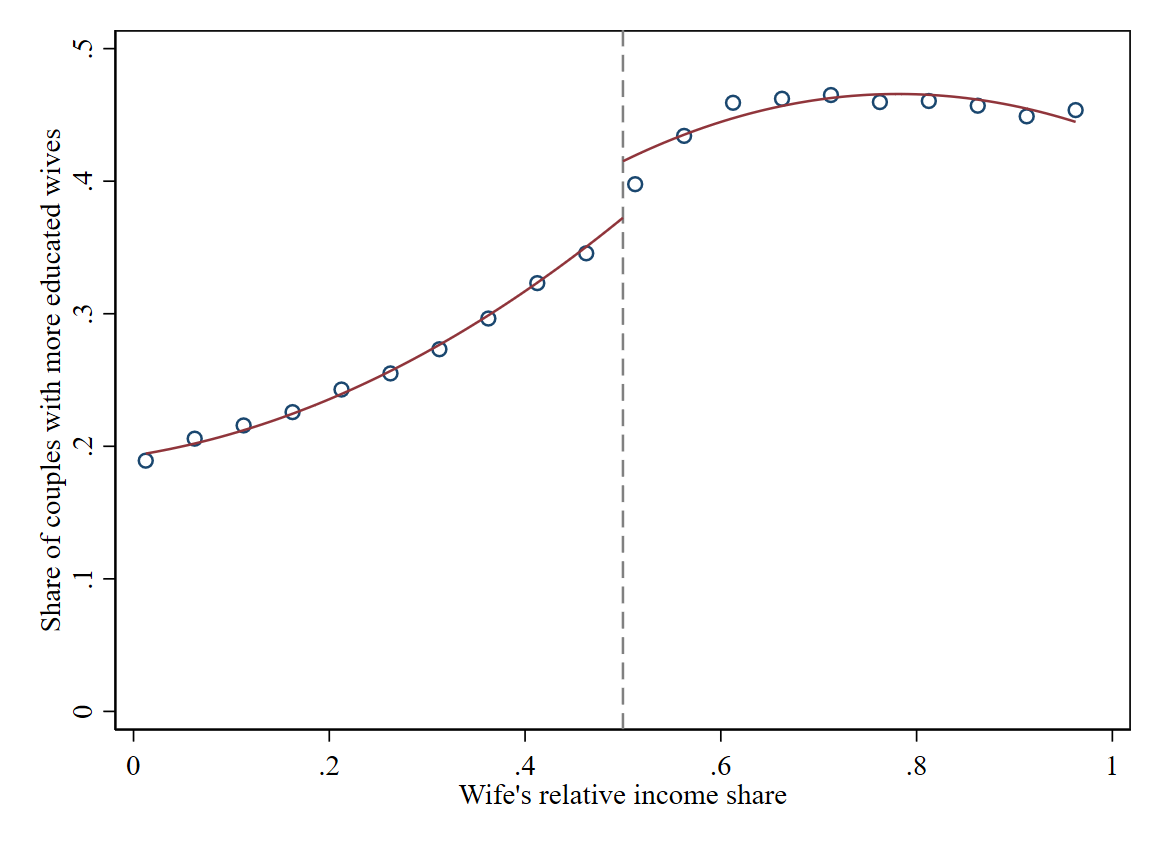
\includegraphics[width=.5\textwidth]{../../results/figures/figure_4.png}
\par \begin{minipage}[h]{\textwidth}{\scriptsize\textit{Notes:} Vertical line marks couples where the woman earns 50\% of the couples income.}\end{minipage}
\end{figure}

	\begin{center}
\begin{adjustbox}{max width=.9\textwidth}
\begin{threeparttable}[H]
\caption{Regression discontinuity estimates: share of couples where the wife has more education}
\label{tab:table_3}
\begin{tabular}{lrrr}
\toprule
\toprule
\textbf{}&\multicolumn{1}{c}{(1)} \\
\midrule
Woman is the highest earner&       0.024\sym{*}  \\
                    &     (0.014)         \\
\midrule Observations&     120.000         \\
\bottomrule
\bottomrule
\end{tabular}
\begin{tablenotes}
\item \footnotesize \textit{Notes:} The regression includes a cubic polynomical of the relative income share, along with interactions between the discontinuity and the polynomial. 
\end{tablenotes}
\end{threeparttable}
\end{adjustbox}
\end{center}

\end{solution}
\end{questions}
\bibliographystyle{apalike}
\bibliography{documents/problem_writeup/bibliography}{}
\end{document}
